% Options for packages loaded elsewhere
\PassOptionsToPackage{unicode}{hyperref}
\PassOptionsToPackage{hyphens}{url}
%
\documentclass[
]{article}
\usepackage{amsmath,amssymb}
\usepackage{lmodern}
\usepackage{iftex}
\ifPDFTeX
  \usepackage[T1]{fontenc}
  \usepackage[utf8]{inputenc}
  \usepackage{textcomp} % provide euro and other symbols
\else % if luatex or xetex
  \usepackage{unicode-math}
  \defaultfontfeatures{Scale=MatchLowercase}
  \defaultfontfeatures[\rmfamily]{Ligatures=TeX,Scale=1}
\fi
% Use upquote if available, for straight quotes in verbatim environments
\IfFileExists{upquote.sty}{\usepackage{upquote}}{}
\IfFileExists{microtype.sty}{% use microtype if available
  \usepackage[]{microtype}
  \UseMicrotypeSet[protrusion]{basicmath} % disable protrusion for tt fonts
}{}
\makeatletter
\@ifundefined{KOMAClassName}{% if non-KOMA class
  \IfFileExists{parskip.sty}{%
    \usepackage{parskip}
  }{% else
    \setlength{\parindent}{0pt}
    \setlength{\parskip}{6pt plus 2pt minus 1pt}}
}{% if KOMA class
  \KOMAoptions{parskip=half}}
\makeatother
\usepackage{xcolor}
\usepackage[margin=1in]{geometry}
\usepackage{color}
\usepackage{fancyvrb}
\newcommand{\VerbBar}{|}
\newcommand{\VERB}{\Verb[commandchars=\\\{\}]}
\DefineVerbatimEnvironment{Highlighting}{Verbatim}{commandchars=\\\{\}}
% Add ',fontsize=\small' for more characters per line
\usepackage{framed}
\definecolor{shadecolor}{RGB}{248,248,248}
\newenvironment{Shaded}{\begin{snugshade}}{\end{snugshade}}
\newcommand{\AlertTok}[1]{\textcolor[rgb]{0.94,0.16,0.16}{#1}}
\newcommand{\AnnotationTok}[1]{\textcolor[rgb]{0.56,0.35,0.01}{\textbf{\textit{#1}}}}
\newcommand{\AttributeTok}[1]{\textcolor[rgb]{0.77,0.63,0.00}{#1}}
\newcommand{\BaseNTok}[1]{\textcolor[rgb]{0.00,0.00,0.81}{#1}}
\newcommand{\BuiltInTok}[1]{#1}
\newcommand{\CharTok}[1]{\textcolor[rgb]{0.31,0.60,0.02}{#1}}
\newcommand{\CommentTok}[1]{\textcolor[rgb]{0.56,0.35,0.01}{\textit{#1}}}
\newcommand{\CommentVarTok}[1]{\textcolor[rgb]{0.56,0.35,0.01}{\textbf{\textit{#1}}}}
\newcommand{\ConstantTok}[1]{\textcolor[rgb]{0.00,0.00,0.00}{#1}}
\newcommand{\ControlFlowTok}[1]{\textcolor[rgb]{0.13,0.29,0.53}{\textbf{#1}}}
\newcommand{\DataTypeTok}[1]{\textcolor[rgb]{0.13,0.29,0.53}{#1}}
\newcommand{\DecValTok}[1]{\textcolor[rgb]{0.00,0.00,0.81}{#1}}
\newcommand{\DocumentationTok}[1]{\textcolor[rgb]{0.56,0.35,0.01}{\textbf{\textit{#1}}}}
\newcommand{\ErrorTok}[1]{\textcolor[rgb]{0.64,0.00,0.00}{\textbf{#1}}}
\newcommand{\ExtensionTok}[1]{#1}
\newcommand{\FloatTok}[1]{\textcolor[rgb]{0.00,0.00,0.81}{#1}}
\newcommand{\FunctionTok}[1]{\textcolor[rgb]{0.00,0.00,0.00}{#1}}
\newcommand{\ImportTok}[1]{#1}
\newcommand{\InformationTok}[1]{\textcolor[rgb]{0.56,0.35,0.01}{\textbf{\textit{#1}}}}
\newcommand{\KeywordTok}[1]{\textcolor[rgb]{0.13,0.29,0.53}{\textbf{#1}}}
\newcommand{\NormalTok}[1]{#1}
\newcommand{\OperatorTok}[1]{\textcolor[rgb]{0.81,0.36,0.00}{\textbf{#1}}}
\newcommand{\OtherTok}[1]{\textcolor[rgb]{0.56,0.35,0.01}{#1}}
\newcommand{\PreprocessorTok}[1]{\textcolor[rgb]{0.56,0.35,0.01}{\textit{#1}}}
\newcommand{\RegionMarkerTok}[1]{#1}
\newcommand{\SpecialCharTok}[1]{\textcolor[rgb]{0.00,0.00,0.00}{#1}}
\newcommand{\SpecialStringTok}[1]{\textcolor[rgb]{0.31,0.60,0.02}{#1}}
\newcommand{\StringTok}[1]{\textcolor[rgb]{0.31,0.60,0.02}{#1}}
\newcommand{\VariableTok}[1]{\textcolor[rgb]{0.00,0.00,0.00}{#1}}
\newcommand{\VerbatimStringTok}[1]{\textcolor[rgb]{0.31,0.60,0.02}{#1}}
\newcommand{\WarningTok}[1]{\textcolor[rgb]{0.56,0.35,0.01}{\textbf{\textit{#1}}}}
\usepackage{graphicx}
\makeatletter
\def\maxwidth{\ifdim\Gin@nat@width>\linewidth\linewidth\else\Gin@nat@width\fi}
\def\maxheight{\ifdim\Gin@nat@height>\textheight\textheight\else\Gin@nat@height\fi}
\makeatother
% Scale images if necessary, so that they will not overflow the page
% margins by default, and it is still possible to overwrite the defaults
% using explicit options in \includegraphics[width, height, ...]{}
\setkeys{Gin}{width=\maxwidth,height=\maxheight,keepaspectratio}
% Set default figure placement to htbp
\makeatletter
\def\fps@figure{htbp}
\makeatother
\setlength{\emergencystretch}{3em} % prevent overfull lines
\providecommand{\tightlist}{%
  \setlength{\itemsep}{0pt}\setlength{\parskip}{0pt}}
\setcounter{secnumdepth}{-\maxdimen} % remove section numbering
\ifLuaTeX
  \usepackage{selnolig}  % disable illegal ligatures
\fi
\IfFileExists{bookmark.sty}{\usepackage{bookmark}}{\usepackage{hyperref}}
\IfFileExists{xurl.sty}{\usepackage{xurl}}{} % add URL line breaks if available
\urlstyle{same} % disable monospaced font for URLs
\hypersetup{
  pdftitle={HW3},
  pdfauthor={ASG},
  hidelinks,
  pdfcreator={LaTeX via pandoc}}

\title{HW3}
\author{ASG}
\date{2023-03-14}

\begin{document}
\maketitle

\hypertarget{section}{%
\subsection{2.6}\label{section}}

\hypertarget{a}{%
\subsubsection{a}\label{a}}

\begin{Shaded}
\begin{Highlighting}[]
\FunctionTok{library}\NormalTok{(RLRsim)}
\end{Highlighting}
\end{Shaded}

\hypertarget{b}{%
\subsubsection{b}\label{b}}

\begin{Shaded}
\begin{Highlighting}[]
\FunctionTok{set.seed}\NormalTok{(}\DecValTok{1}\NormalTok{)}
\NormalTok{x }\OtherTok{\textless{}{-}} \FunctionTok{seq}\NormalTok{(}\DecValTok{0}\NormalTok{,}\DecValTok{1}\NormalTok{,}\AttributeTok{length =} \DecValTok{200}\NormalTok{)}
\NormalTok{y }\OtherTok{\textless{}{-}}\NormalTok{ x }\SpecialCharTok{+} \FunctionTok{rnorm}\NormalTok{(}\DecValTok{200}\NormalTok{)}
\end{Highlighting}
\end{Shaded}

\hypertarget{c}{%
\subsubsection{c}\label{c}}

\begin{Shaded}
\begin{Highlighting}[]
\FunctionTok{library}\NormalTok{(mgcv) ; }\FunctionTok{library}\NormalTok{(RLRsim)}
\NormalTok{fitLine }\OtherTok{\textless{}{-}} \FunctionTok{gam}\NormalTok{(y }\SpecialCharTok{\textasciitilde{}}\NormalTok{ x) ; fitDfltPenSpl }\OtherTok{\textless{}{-}} \FunctionTok{gam}\NormalTok{(y }\SpecialCharTok{\textasciitilde{}} \FunctionTok{s}\NormalTok{(x))}
\FunctionTok{print}\NormalTok{(}\FunctionTok{anova}\NormalTok{(fitLine,fitDfltPenSpl,}\AttributeTok{test =} \StringTok{"F"}\NormalTok{)}\SpecialCharTok{$}\StringTok{"Pr(\textgreater{}F)"}\NormalTok{[}\DecValTok{2}\NormalTok{])}
\end{Highlighting}
\end{Shaded}

\begin{verbatim}
## [1] 7.514685e-09
\end{verbatim}

\begin{Shaded}
\begin{Highlighting}[]
\NormalTok{fitOLSspl }\OtherTok{\textless{}{-}} \FunctionTok{gam}\NormalTok{(y }\SpecialCharTok{\textasciitilde{}} \FunctionTok{s}\NormalTok{(x,}\AttributeTok{k =} \DecValTok{5}\NormalTok{,}\AttributeTok{sp =} \DecValTok{0}\NormalTok{))}
\FunctionTok{print}\NormalTok{(}\FunctionTok{anova}\NormalTok{(fitLine,fitOLSspl,}\AttributeTok{test =} \StringTok{"F"}\NormalTok{)}\SpecialCharTok{$}\StringTok{"Pr(\textgreater{}F)"}\NormalTok{[}\DecValTok{2}\NormalTok{])}
\end{Highlighting}
\end{Shaded}

\begin{verbatim}
## [1] 0.6872285
\end{verbatim}

\begin{Shaded}
\begin{Highlighting}[]
\NormalTok{fitGAMM }\OtherTok{\textless{}{-}} \FunctionTok{gamm}\NormalTok{(y }\SpecialCharTok{\textasciitilde{}} \FunctionTok{s}\NormalTok{(x),}\AttributeTok{method =} \StringTok{"REML"}\NormalTok{)}
\FunctionTok{print}\NormalTok{(}\FunctionTok{exactRLRT}\NormalTok{(fitGAMM}\SpecialCharTok{$}\NormalTok{lme)[}\DecValTok{2}\NormalTok{])}
\end{Highlighting}
\end{Shaded}

\begin{verbatim}
## $p.value
## [1] 1
\end{verbatim}

If the p value is high, we accept the null hypothesis. In this case, 2
tests shows high p-value hence we do not reject the null hypothesis for
data generated when seed=1. Since H0 is true , and for two tests we get
high p-value , we can say that the OLS and RLRT test are veritable test
and F game test is not.

\hypertarget{d}{%
\subsubsection{d}\label{d}}

\begin{Shaded}
\begin{Highlighting}[]
\NormalTok{sample}\OtherTok{\textless{}{-}}\DecValTok{1000}
\NormalTok{Fgam}\OtherTok{\textless{}{-}}\FunctionTok{c}\NormalTok{()}
\NormalTok{Fols}\OtherTok{\textless{}{-}}\FunctionTok{c}\NormalTok{()}
\NormalTok{RLRT}\OtherTok{\textless{}{-}}\FunctionTok{c}\NormalTok{()}
\ControlFlowTok{for}\NormalTok{ (i }\ControlFlowTok{in} \DecValTok{1}\SpecialCharTok{:}\NormalTok{sample)\{}
  \FunctionTok{set.seed}\NormalTok{(i)}
\NormalTok{  x }\OtherTok{\textless{}{-}} \FunctionTok{seq}\NormalTok{(}\DecValTok{0}\NormalTok{,}\DecValTok{1}\NormalTok{,}\AttributeTok{length =} \DecValTok{200}\NormalTok{)}
\NormalTok{  y }\OtherTok{\textless{}{-}}\NormalTok{ x }\SpecialCharTok{+} \FunctionTok{rnorm}\NormalTok{(}\DecValTok{200}\NormalTok{)}
  
\NormalTok{  fitLine }\OtherTok{\textless{}{-}} \FunctionTok{gam}\NormalTok{(y }\SpecialCharTok{\textasciitilde{}}\NormalTok{ x) ; fitDfltPenSpl }\OtherTok{\textless{}{-}} \FunctionTok{gam}\NormalTok{(y }\SpecialCharTok{\textasciitilde{}} \FunctionTok{s}\NormalTok{(x))}
\NormalTok{  Fgam[i]}\OtherTok{\textless{}{-}}\FunctionTok{anova}\NormalTok{(fitLine,fitDfltPenSpl,}\AttributeTok{test =} \StringTok{"F"}\NormalTok{)}\SpecialCharTok{$}\StringTok{"Pr(\textgreater{}F)"}\NormalTok{[}\DecValTok{2}\NormalTok{]}
  
\NormalTok{  fitOLSspl }\OtherTok{\textless{}{-}} \FunctionTok{gam}\NormalTok{(y }\SpecialCharTok{\textasciitilde{}} \FunctionTok{s}\NormalTok{(x,}\AttributeTok{k =} \DecValTok{5}\NormalTok{,}\AttributeTok{sp =} \DecValTok{0}\NormalTok{))}
\NormalTok{  Fols[i]}\OtherTok{\textless{}{-}}\FunctionTok{anova}\NormalTok{(fitLine,fitOLSspl,}\AttributeTok{test =} \StringTok{"F"}\NormalTok{)}\SpecialCharTok{$}\StringTok{"Pr(\textgreater{}F)"}\NormalTok{[}\DecValTok{2}\NormalTok{]}
  
\NormalTok{  fitGAMM }\OtherTok{\textless{}{-}} \FunctionTok{gamm}\NormalTok{(y }\SpecialCharTok{\textasciitilde{}} \FunctionTok{s}\NormalTok{(x),}\AttributeTok{method =} \StringTok{"REML"}\NormalTok{)}
\NormalTok{  RLRT[i]}\OtherTok{\textless{}{-}}\FunctionTok{exactRLRT}\NormalTok{(fitGAMM}\SpecialCharTok{$}\NormalTok{lme)[}\DecValTok{2}\NormalTok{]}\SpecialCharTok{$}\NormalTok{p.value}
  
\NormalTok{\}}
\FunctionTok{hist}\NormalTok{(Fgam)}
\end{Highlighting}
\end{Shaded}

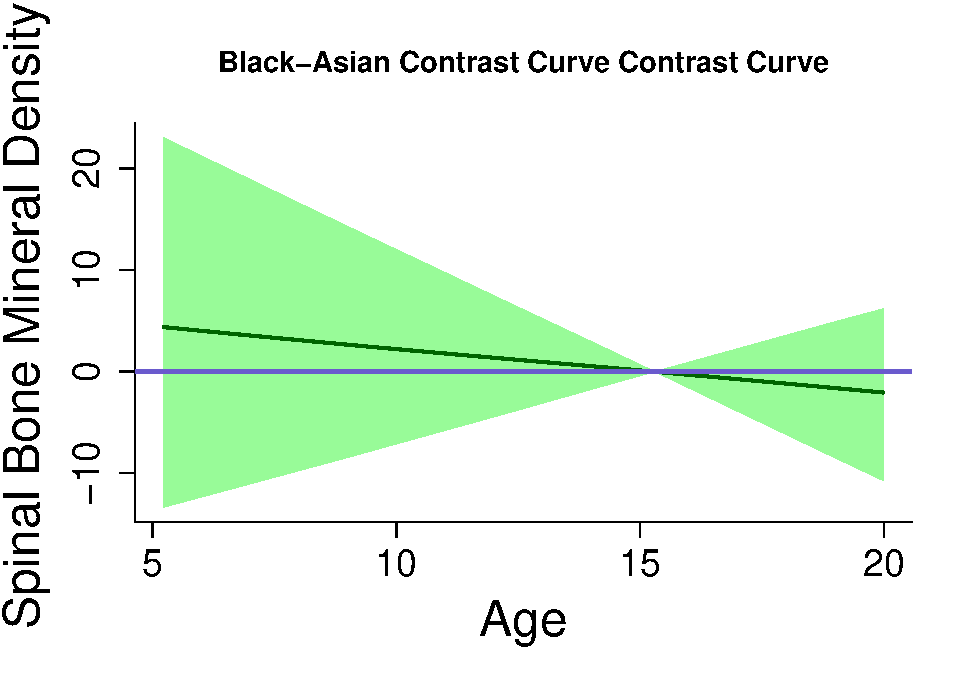
\includegraphics{HW3_files/figure-latex/unnamed-chunk-4-1.pdf}

\begin{Shaded}
\begin{Highlighting}[]
\FunctionTok{hist}\NormalTok{(Fols)}
\end{Highlighting}
\end{Shaded}

\includegraphics{HW3_files/figure-latex/unnamed-chunk-4-2.pdf}

\begin{Shaded}
\begin{Highlighting}[]
\FunctionTok{hist}\NormalTok{(RLRT)}
\end{Highlighting}
\end{Shaded}

\includegraphics{HW3_files/figure-latex/unnamed-chunk-4-3.pdf} Gam F
test: The distribution of pvalues of this particular test is a left
skewed distribution. Hence we can conclude that this F test usually
rejects the null hypothesis that f is linear. The bulk of the simulation
yielded pvalues well below the standard significance level of 0.05

OLS F test: The p values from this histogram is more normally
distributed. Hence we can conclude that the pvalues are higher generally
hence we should accept the null hypothesis.

RLRT : The p values are usually 1 in this case. Which means that the
observed test statistic is 0 for more than half the sample dataset. Thus
we can say that the null hypothesis is usually accepted. This is because
according to RLRT for most of the test the H0 And H1 were
indistinguishable and for the rest , we still get high p values when
significance level is set to 0.05.

\hypertarget{e}{%
\subsubsection{e}\label{e}}

\begin{Shaded}
\begin{Highlighting}[]
\NormalTok{Fgamprobs}\OtherTok{\textless{}{-}}\FunctionTok{length}\NormalTok{(}\FunctionTok{which}\NormalTok{(Fgam}\SpecialCharTok{\textless{}}\FloatTok{0.05}\NormalTok{))}\SpecialCharTok{/}\FunctionTok{length}\NormalTok{(Fgam)}
\FunctionTok{print}\NormalTok{(Fgamprobs)}
\end{Highlighting}
\end{Shaded}

\begin{verbatim}
## [1] 0.644
\end{verbatim}

\begin{Shaded}
\begin{Highlighting}[]
\NormalTok{Folsprobs}\OtherTok{\textless{}{-}}\FunctionTok{length}\NormalTok{(}\FunctionTok{which}\NormalTok{(Fols}\SpecialCharTok{\textless{}}\FloatTok{0.05}\NormalTok{))}\SpecialCharTok{/}\FunctionTok{length}\NormalTok{(Fols)}
\FunctionTok{print}\NormalTok{(Folsprobs)}
\end{Highlighting}
\end{Shaded}

\begin{verbatim}
## [1] 0.045
\end{verbatim}

\begin{Shaded}
\begin{Highlighting}[]
\NormalTok{RLRTprobs}\OtherTok{\textless{}{-}}\FunctionTok{length}\NormalTok{(}\FunctionTok{which}\NormalTok{(RLRT}\SpecialCharTok{\textless{}}\FloatTok{0.05}\NormalTok{))}\SpecialCharTok{/}\FunctionTok{length}\NormalTok{(RLRT)}
\FunctionTok{print}\NormalTok{(RLRTprobs)}
\end{Highlighting}
\end{Shaded}

\begin{verbatim}
## [1] 0.044
\end{verbatim}

The F OLS test and the RLRT test have the probability closer to the
advertised significance level.

\hypertarget{section-1}{%
\subsection{2.7}\label{section-1}}

\hypertarget{a-1}{%
\subsubsection{a}\label{a-1}}

\begin{Shaded}
\begin{Highlighting}[]
\NormalTok{theta }\OtherTok{\textless{}{-}} \FunctionTok{seq}\NormalTok{(}\DecValTok{0}\NormalTok{,}\DecValTok{1}\NormalTok{,}\AttributeTok{by =} \FloatTok{0.05}\NormalTok{)}
\NormalTok{xg }\OtherTok{\textless{}{-}} \FunctionTok{seq}\NormalTok{(}\DecValTok{0}\NormalTok{,}\DecValTok{1}\NormalTok{,}\AttributeTok{length =} \DecValTok{1001}\NormalTok{)}
\FunctionTok{plot}\NormalTok{(xg,xg,}\AttributeTok{type=}\StringTok{"l"}\NormalTok{,}\AttributeTok{ylim =} \FunctionTok{c}\NormalTok{(}\DecValTok{0}\NormalTok{,}\FloatTok{2.15}\NormalTok{),}\AttributeTok{bty =} \StringTok{"l"}\NormalTok{,}\AttributeTok{xlab =} \StringTok{"x"}\NormalTok{,}\AttributeTok{ylab =} \FunctionTok{expression}\NormalTok{(}\FunctionTok{paste}\NormalTok{(}\StringTok{"f(x;"}\NormalTok{,theta,}\StringTok{")"}\NormalTok{)))}
\ControlFlowTok{for}\NormalTok{ (j }\ControlFlowTok{in} \DecValTok{2}\SpecialCharTok{:}\FunctionTok{length}\NormalTok{(theta)) }\FunctionTok{lines}\NormalTok{(xg,xg }\SpecialCharTok{+}\NormalTok{ theta[j]}\SpecialCharTok{*}\FunctionTok{dnorm}\NormalTok{(xg,}\FloatTok{0.5}\NormalTok{,}\FloatTok{0.25}\NormalTok{),}\AttributeTok{col =}\NormalTok{ j)}
\end{Highlighting}
\end{Shaded}

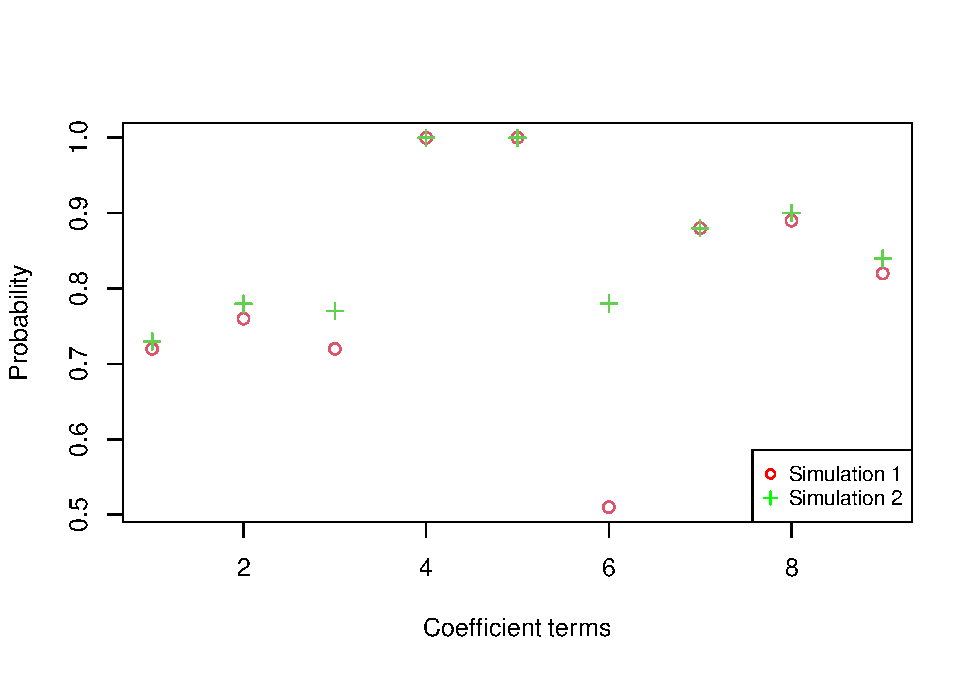
\includegraphics{HW3_files/figure-latex/unnamed-chunk-6-1.pdf}

\hypertarget{b-1}{%
\subsubsection{b}\label{b-1}}

\begin{Shaded}
\begin{Highlighting}[]
\NormalTok{get\_power }\OtherTok{\textless{}{-}} \ControlFlowTok{function}\NormalTok{(theta, }\AttributeTok{sample=}\DecValTok{1000}\NormalTok{)\{}
\NormalTok{  Fgam}\OtherTok{\textless{}{-}}\FunctionTok{c}\NormalTok{()}
\NormalTok{  Fols}\OtherTok{\textless{}{-}}\FunctionTok{c}\NormalTok{()}
\NormalTok{  RLRT}\OtherTok{\textless{}{-}}\FunctionTok{c}\NormalTok{()}
  \ControlFlowTok{for}\NormalTok{ (i }\ControlFlowTok{in} \DecValTok{1}\SpecialCharTok{:}\NormalTok{sample)\{}
    \FunctionTok{set.seed}\NormalTok{(i)}
\NormalTok{    x }\OtherTok{\textless{}{-}} \FunctionTok{seq}\NormalTok{(}\DecValTok{0}\NormalTok{,}\DecValTok{1}\NormalTok{,}\AttributeTok{length =} \DecValTok{200}\NormalTok{)}
\NormalTok{    y }\OtherTok{\textless{}{-}}\NormalTok{ x }\SpecialCharTok{+}\NormalTok{ theta}\SpecialCharTok{*}\FunctionTok{dnorm}\NormalTok{(x,}\FloatTok{0.5}\NormalTok{,}\FloatTok{0.25}\NormalTok{) }\SpecialCharTok{+} \FunctionTok{rnorm}\NormalTok{(}\DecValTok{200}\NormalTok{)}
    
\NormalTok{    fitLine }\OtherTok{\textless{}{-}} \FunctionTok{gam}\NormalTok{(y }\SpecialCharTok{\textasciitilde{}}\NormalTok{ x) ; fitDfltPenSpl }\OtherTok{\textless{}{-}} \FunctionTok{gam}\NormalTok{(y }\SpecialCharTok{\textasciitilde{}} \FunctionTok{s}\NormalTok{(x))}
\NormalTok{    Fgam[i]}\OtherTok{\textless{}{-}}\FunctionTok{anova}\NormalTok{(fitLine,fitDfltPenSpl,}\AttributeTok{test =} \StringTok{"F"}\NormalTok{)}\SpecialCharTok{$}\StringTok{"Pr(\textgreater{}F)"}\NormalTok{[}\DecValTok{2}\NormalTok{]}
    
\NormalTok{    fitOLSspl }\OtherTok{\textless{}{-}} \FunctionTok{gam}\NormalTok{(y }\SpecialCharTok{\textasciitilde{}} \FunctionTok{s}\NormalTok{(x,}\AttributeTok{k =} \DecValTok{5}\NormalTok{,}\AttributeTok{sp =} \DecValTok{0}\NormalTok{))}
\NormalTok{    Fols[i]}\OtherTok{\textless{}{-}}\FunctionTok{anova}\NormalTok{(fitLine,fitOLSspl,}\AttributeTok{test =} \StringTok{"F"}\NormalTok{)}\SpecialCharTok{$}\StringTok{"Pr(\textgreater{}F)"}\NormalTok{[}\DecValTok{2}\NormalTok{]}
    
\NormalTok{    fitGAMM }\OtherTok{\textless{}{-}} \FunctionTok{gamm}\NormalTok{(y }\SpecialCharTok{\textasciitilde{}} \FunctionTok{s}\NormalTok{(x),}\AttributeTok{method =} \StringTok{"REML"}\NormalTok{)}
\NormalTok{    RLRT[i]}\OtherTok{\textless{}{-}}\FunctionTok{exactRLRT}\NormalTok{(fitGAMM}\SpecialCharTok{$}\NormalTok{lme)[}\DecValTok{2}\NormalTok{]}\SpecialCharTok{$}\NormalTok{p.value}
    
\NormalTok{  \}}
\NormalTok{  Fgamprobs}\OtherTok{\textless{}{-}}\FunctionTok{length}\NormalTok{(}\FunctionTok{which}\NormalTok{(Fgam}\SpecialCharTok{\textless{}}\FloatTok{0.05}\NormalTok{))}\SpecialCharTok{/}\FunctionTok{length}\NormalTok{(Fgam)}
\NormalTok{  Folsprobs}\OtherTok{\textless{}{-}}\FunctionTok{length}\NormalTok{(}\FunctionTok{which}\NormalTok{(Fols}\SpecialCharTok{\textless{}}\FloatTok{0.05}\NormalTok{))}\SpecialCharTok{/}\FunctionTok{length}\NormalTok{(Fols)}
\NormalTok{  RLRTprobs}\OtherTok{\textless{}{-}}\FunctionTok{length}\NormalTok{(}\FunctionTok{which}\NormalTok{(RLRT}\SpecialCharTok{\textless{}}\FloatTok{0.05}\NormalTok{))}\SpecialCharTok{/}\FunctionTok{length}\NormalTok{(RLRT)}
  \FunctionTok{return}\NormalTok{(}\FunctionTok{c}\NormalTok{(Fgamprobs,Folsprobs, RLRTprobs))}
\NormalTok{\}}

\NormalTok{theta }\OtherTok{\textless{}{-}} \FunctionTok{seq}\NormalTok{(}\DecValTok{0}\NormalTok{,}\DecValTok{1}\NormalTok{,}\AttributeTok{by =} \FloatTok{0.05}\NormalTok{)}
\NormalTok{power}\OtherTok{\textless{}{-}}\FunctionTok{c}\NormalTok{()}
\ControlFlowTok{for}\NormalTok{ (i }\ControlFlowTok{in} \DecValTok{2}\SpecialCharTok{:}\FunctionTok{length}\NormalTok{(theta))\{}
\NormalTok{  power}\OtherTok{\textless{}{-}}\FunctionTok{rbind}\NormalTok{(power,}\FunctionTok{get\_power}\NormalTok{(theta[i],}\DecValTok{1000}\NormalTok{))}
\NormalTok{\}}
\NormalTok{power}\OtherTok{\textless{}{-}}\FunctionTok{data.frame}\NormalTok{(}\FunctionTok{cbind}\NormalTok{(power,theta))}

\FunctionTok{plot}\NormalTok{(theta,theta,}\AttributeTok{ylim =} \FunctionTok{c}\NormalTok{(}\DecValTok{0}\NormalTok{,}\FloatTok{2.15}\NormalTok{),}\AttributeTok{bty =} \StringTok{"l"}\NormalTok{)}
\FunctionTok{lines}\NormalTok{(power}\SpecialCharTok{$}\NormalTok{theta,power}\SpecialCharTok{$}\NormalTok{V1,}\AttributeTok{col=}\StringTok{"red"}\NormalTok{,}\AttributeTok{lty=}\DecValTok{1}\NormalTok{,}\AttributeTok{lwd=}\DecValTok{2}\NormalTok{)}
\FunctionTok{lines}\NormalTok{(power}\SpecialCharTok{$}\NormalTok{theta,power}\SpecialCharTok{$}\NormalTok{V2,}\AttributeTok{col=}\StringTok{"blue"}\NormalTok{,}\AttributeTok{lty=}\DecValTok{2}\NormalTok{,}\AttributeTok{lwd=}\DecValTok{2}\NormalTok{)}
\FunctionTok{lines}\NormalTok{(power}\SpecialCharTok{$}\NormalTok{theta,power}\SpecialCharTok{$}\NormalTok{V3,}\AttributeTok{col=}\StringTok{"green"}\NormalTok{,}\AttributeTok{lty=}\DecValTok{3}\NormalTok{,}\AttributeTok{lwd=}\DecValTok{2}\NormalTok{)}
\FunctionTok{legend}\NormalTok{(}\StringTok{\textquotesingle{}topright\textquotesingle{}}\NormalTok{,}\AttributeTok{legend=}\FunctionTok{c}\NormalTok{(}\StringTok{"F gam test"}\NormalTok{,}\StringTok{"F ols test"}\NormalTok{,}\StringTok{"RLRT"}\NormalTok{),}\AttributeTok{col=}\FunctionTok{c}\NormalTok{(}\StringTok{"red"}\NormalTok{,}\StringTok{"blue"}\NormalTok{,}\StringTok{"green"}\NormalTok{),}\AttributeTok{lty=}\DecValTok{1}\SpecialCharTok{:}\DecValTok{2}\NormalTok{, }\AttributeTok{cex=}\FloatTok{0.6}\NormalTok{)}
\end{Highlighting}
\end{Shaded}

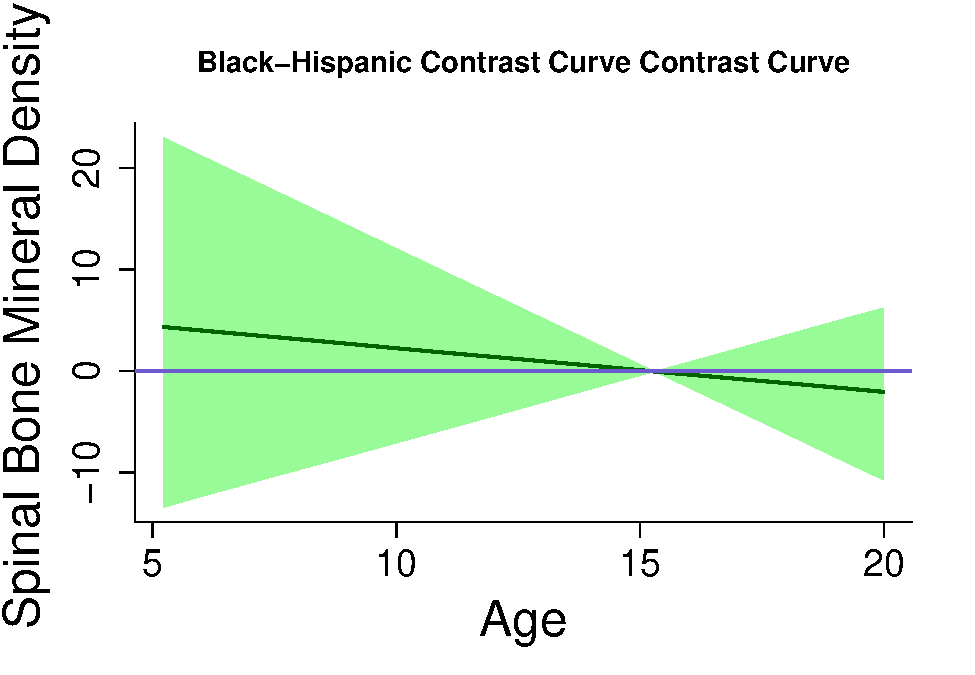
\includegraphics{HW3_files/figure-latex/unnamed-chunk-7-1.pdf} \#\#\# e

As the theta increases, the ols and rlrt correctly rejects the null
hypothesis and provides a higher rejection probability. while the F gam
test doesnt seem to have similar trend and has higher rejection
probability even when theta is near 0(linearity indicator). Thus F ols
test and rlrt test are much better test in response and the rlrt proves
to be a much powerful test as it provides higher rejection probability
as theta increases.

\hypertarget{section-2}{%
\subsection{3}\label{section-2}}

\hypertarget{a-2}{%
\subsubsection{a}\label{a-2}}

The dataset used is a time series data in the default Dataset package of
r called as ldeaths. It measures the lung related mortality rate in UK
residents. The official description is as follows: ``Three time series
giving the monthly deaths from bronchitis, emphysema and asthma in the
UK, 1974--1979, both sexes (ldeaths), males (mdeaths) and females
(fdeaths).'' the mentioned source is : ``P. J. Diggle (1990) Time
Series: A Biostatistical Introduction. Oxford, table A.3''

\hypertarget{b-2}{%
\subsubsection{b}\label{b-2}}

The regressor variable is Date. The data is collected monthly between
1974 to 1979 The response variable is number of deaths from lung
diseases in UK residents.

\hypertarget{c-1}{%
\subsubsection{c}\label{c-1}}

\begin{Shaded}
\begin{Highlighting}[]
\FunctionTok{library}\NormalTok{(datasets)}
\NormalTok{ldeath}\OtherTok{\textless{}{-}}\FunctionTok{data.frame}\NormalTok{(}\AttributeTok{Y=}\FunctionTok{as.matrix}\NormalTok{(ldeaths), }\AttributeTok{date=}\NormalTok{zoo}\SpecialCharTok{::}\FunctionTok{as.Date}\NormalTok{(}\FunctionTok{time}\NormalTok{(ldeaths)))}
\NormalTok{x }\OtherTok{\textless{}{-}} \FunctionTok{as.numeric}\NormalTok{(ldeath}\SpecialCharTok{$}\NormalTok{date)}
\NormalTok{y }\OtherTok{\textless{}{-}}\NormalTok{ ldeath}\SpecialCharTok{$}\NormalTok{Y}
\FunctionTok{plot}\NormalTok{(ldeath}\SpecialCharTok{$}\NormalTok{date,y,}\AttributeTok{bty =} \StringTok{"l"}\NormalTok{,}\AttributeTok{col =} \StringTok{"dodgerblue"}\NormalTok{)}
\NormalTok{fitGAMcr}\OtherTok{\textless{}{-}}\FunctionTok{gam}\NormalTok{(y }\SpecialCharTok{\textasciitilde{}} \FunctionTok{s}\NormalTok{(x,}\AttributeTok{bs =} \StringTok{"cr"}\NormalTok{,}\AttributeTok{k=}\DecValTok{25}\NormalTok{))}
\NormalTok{xg }\OtherTok{\textless{}{-}} \FunctionTok{seq}\NormalTok{(}\FunctionTok{min}\NormalTok{(x),}\FunctionTok{max}\NormalTok{(x),}\AttributeTok{length =} \DecValTok{1000}\NormalTok{)}
\NormalTok{fHatgGAMcr }\OtherTok{\textless{}{-}} \FunctionTok{predict}\NormalTok{(fitGAMcr,}\AttributeTok{newdata =} \FunctionTok{data.frame}\NormalTok{(}\AttributeTok{x =}\NormalTok{ xg))}
\FunctionTok{lines}\NormalTok{(xg,fHatgGAMcr,}\AttributeTok{col =} \StringTok{"darkgreen"}\NormalTok{,}\AttributeTok{lwd=}\DecValTok{2}\NormalTok{)}
\end{Highlighting}
\end{Shaded}

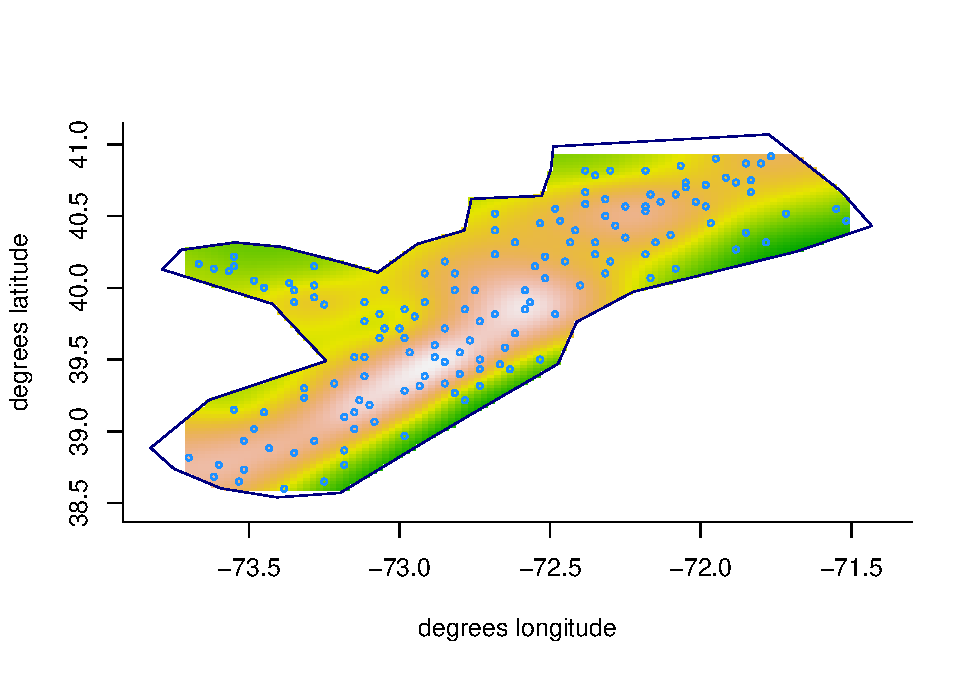
\includegraphics{HW3_files/figure-latex/unnamed-chunk-8-1.pdf}

\begin{Shaded}
\begin{Highlighting}[]
\FunctionTok{gam.check}\NormalTok{(fitGAMcr)}
\end{Highlighting}
\end{Shaded}

\includegraphics{HW3_files/figure-latex/unnamed-chunk-8-2.pdf}

\begin{verbatim}
## 
## Method: GCV   Optimizer: magic
## Smoothing parameter selection converged after 6 iterations.
## The RMS GCV score gradient at convergence was 9.152286 .
## The Hessian was positive definite.
## Model rank =  25 / 25 
## 
## Basis dimension (k) checking results. Low p-value (k-index<1) may
## indicate that k is too low, especially if edf is close to k'.
## 
##      k' edf k-index p-value
## s(x) 24  20    0.99     0.4
\end{verbatim}

\hypertarget{d-1}{%
\subsubsection{d}\label{d-1}}

The model complexity is fairly high for this dataset. I started out
without setting the K value and used gam.check to find optimal K. it
gave result as 10. i tried using k from 12 to 25 to check which fits the
plot better. K=25 the actual vs fitted plot was fairly linear, which
means the model was performing good. Hence the GAM was very robustly
able to model such a time series data which had periodic properties.

\end{document}
